\documentclass{ctexart}
\usepackage{PhysicalChemistryNote}

\begin{document}\pagestyle{plain}
\noindent\tbf{\LARGE 6A 电解质溶液}\vspace{15pt}\\
\indent 电解质溶液,例如食盐水,具有普通溶液所不具有的导电性,%
这是因为溶液中的\ce{Na^+}和\ce{Cl^-}在电场的作用下能发生定向移动,起到传递电荷的作用.%
除此之外,带异种电荷的离子之间还存在吸引力,带同种电荷的离子之间还存在排斥力.%
以上种种原因,都使得电解质溶液与一般的溶液性质并不完全相似.因此,%
我们将在本节简单的讨论其性质.\vspace{12pt}\\
\Section{6A.1 电解质溶液的电导}
\Part{电导,电导率和摩尔电导率}
\indent 物质的导电能力,通常用电阻$R$来表示.而对于电解质溶液,我们更希望直观地判断其导电能力,%
这一物理量越大,电解质溶液的导电能力就越强.因此,可以定义\tbf{电导}来衡量其导电能力.
\begin{definition}[6A.1.1 电导]
    \tbf{电导}$G$定义为电阻$R$的倒数,即$G=\dfrac1R$.
\end{definition}
导体的电阻与其长度$l$成正比,与其横截面积$S$成反比,比例系数为电阻率$\rho$,它与导体的材料有关.于是
\[R=\rho\dfrac{l}{S}\]
因此,物体的电导
\[G=\dfrac{1}{\rho}\dfrac{S}{l}\]
同样地,可以定义\tbf{电导率}以衡量材料的导电能力.
\begin{definition}[6A.1.2 电导率]
    \tbf{电导率}$\kappa$定义为电阻率$\rho$的倒数,即$\kappa=\dfrac{1}{\rho}$.
\end{definition}
对于不同浓度的溶液,其中离子的数目不同,因而导电性也是不同的.%
因此,可以定义\tbf{摩尔电导率}.
\begin{definition}[6A.1.3 摩尔电导率]
    \tbf{摩尔电导率}$\Lambda_\m$定义为溶液电阻率与摩尔浓度的之比,即$\Lambda_\m=\dfrac{\kappa}{c}$.\\
    摩尔电导率的操作定义\footnotemark 为在两个相距$1\text{ m}$的平行电极板之间充入含有$1\mol$电解质的一定浓度的溶液时具有的电导.
\end{definition}\footnotetext{操作定义,是根据可观察,可测量,可操作的特征来界定变量含义的方法.}
在讨论摩尔电导率时,需要指定电解质的基本单元.例如$\Lambda_\m(\ce{NaCl})$和$\displaystyle\Lambda_\m\left(\ce{1/2NaCl}\right)$%
在操作定义中分别指\ce{NaCl}为$1\mol$和\ce{Na^+}与\ce{Cl^-}的总量为$1\mol$.对于同一浓度的\ce{NaCl}溶液,有
\[\Lambda_\m(\ce{NaCl})=2\Lambda_\m\left(\ce{1/2NaCl}\right)\]
\Part{电导率,摩尔电导率与浓度的关系}
\indent 我们先讨论浓度与电导率的关系.几种典型的电解质溶液的电导率与浓度的关系如下图所示.
\begin{tightcenter}
    \documentclass{standalone}
\usepackage{PhysicalChemistryNote}
\begin{document}
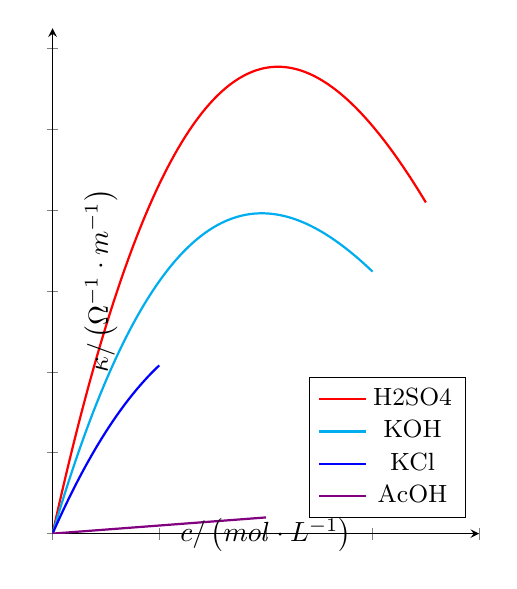
\begin{tikzpicture}
    \begin{axis}[
        width = 7cm,
        height = 8cm,
        legend pos = south east,
        xlabel = {$c/\left(\text{mol}\cdot\text{L}^{-1}\right)$},
        ylabel = {$\kappa/\left(\Omega^{-1}\cdot\text{m}^{-1}\right)$},
        axis lines = left,
        x label style={at={(axis description cs:0.5,0.05)},anchor=north},
        y label style={at={(axis description cs:0.175,0.5)},rotate=0,anchor=south},
        ymax = 1.25,
        ymin = 0,
        xmax = 0.8,
        ymin = 0,
        samples = 400,
        xticklabels={},
        yticklabels={}
    ]
    \addplot [thick, red, domain=0:0.7] {3*x*(x-1)*(x-2)};
    \addlegendentry{\small{\ce{H2SO4}}}
    \addplot [thick, cyan, domain=0:0.6] {3*x*(x-1)*(x-1.5)};
    \addlegendentry{\small{\ce{KOH}}}
    \addplot [thick, blue, domain=0:0.2] {2*x*(x-1)*(x-1.5)};
    \addlegendentry{\small{\ce{KCl}}}
    \addplot [thick, violet, domain=0:0.4] {0.1*x};
    \addlegendentry{\small{\ce{AcOH}}}
    \end{axis}
\end{tikzpicture}
\end{document}
\end{tightcenter}
可以看出,在一定浓度范围内,强电解质的电导率$\kappa$随浓度的上升而上升,%
这是由于溶液中离子的浓度上升使得导电的粒子数增多;超过一定浓度范围后,$\kappa$随浓度增大而减小,%
这是由于离子变得密集,正负离子间的吸引力增大,限制了离子的导电能力所致.\\
\indent 对于弱电解质而言,$\kappa$随浓度变化不显著.浓度增大,虽然单位体积溶液的电解质分子数增多,%
但电离度却随之减小,因此离子的浓度变化不大.\\
\indent 与电导率所不同,电解质的摩尔电导率$\Lambda_\m$却总是随着浓度的增加而减小.%
几种典型的电解质溶液的电导率与浓度的关系如下图所示.
\end{document}